% LTeX: language=zh-CN
% TODO LIST
% 第一章 绪论
% 二维材料及其异质结
%%% 背景
%%%% 二维材料
%%%% 二维材料异质结
%%%% 实验现状
%%%% 理论现状
\chapter{绪\hspace{6pt}论}

\section{二维材料及其异质结概述}
\subsection{二维材料概述}
    自从石墨烯被发现并且成功大规模制备以来\citing{RN1023-2004,RN801-2009},二维体系中的出现的大量新型二维材料已经引起了许多研究者的持续关注。由于二维材料所具有的独特电子结构、不同寻常的声光耦合、奇异的层间作用已经多样化的结构性质调控手段,在许多新型电子、光电子器件中不同种类的二维材料发挥着重要作用。现如今,包括石墨烯在内的多种体系的二维材料被理论上预言并在成功的实验中制备,例如与石墨烯具有相似晶格结构的六方氮化硼(Hexagonal boron nitride,h-BN),具有折叠晶格结构的黑鳞(Black phosphorus,BP),具有多种二维相的过渡族金属硫族化合物(Transition metal dichalcogenides, TMDS)以及二维金属氧化物(Metal oxides),二维三五族半导体(III-V component semiconductors, III-Vs)等。这些不同二维材料来源于各自不同的材料体系,具有各自截然不同的物理性质和化学性质。%//TODO 引用

    \begin{figure}[htb]
        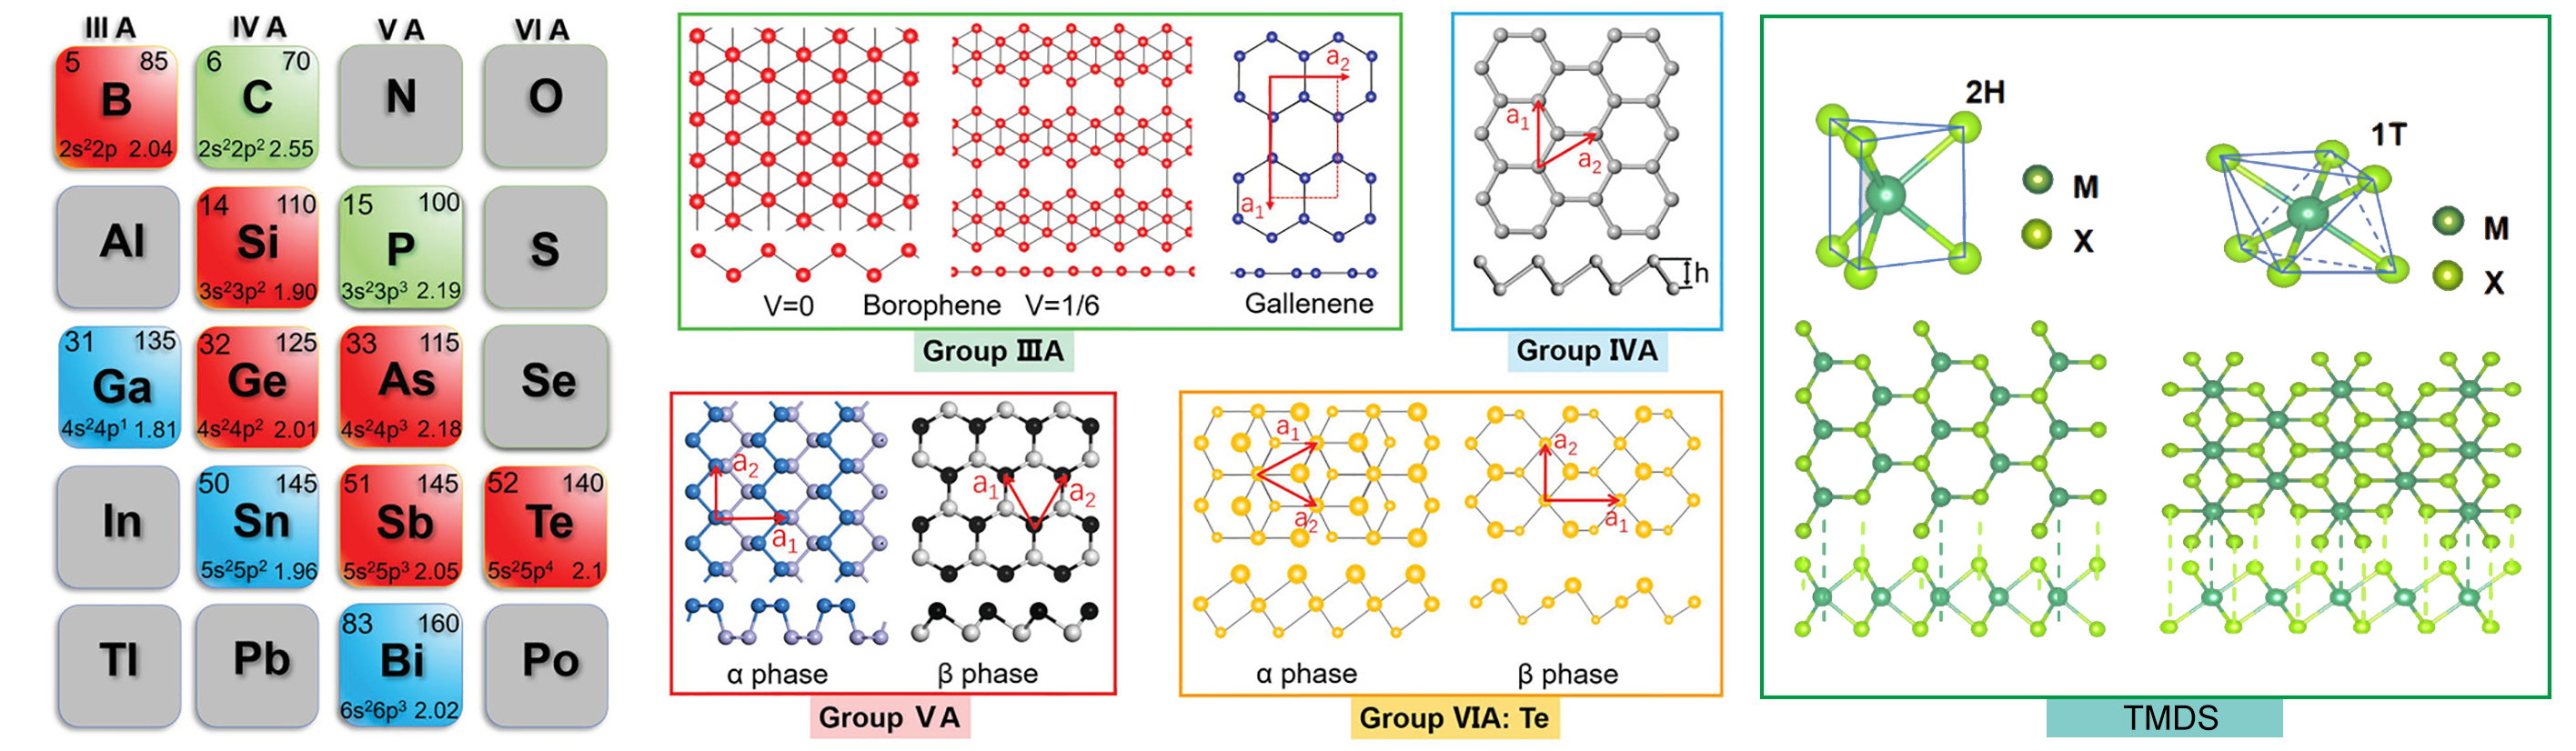
\includegraphics[width=0.8\textwidth]{pic/INTRO_ALL_monoelement_2DM.png}
        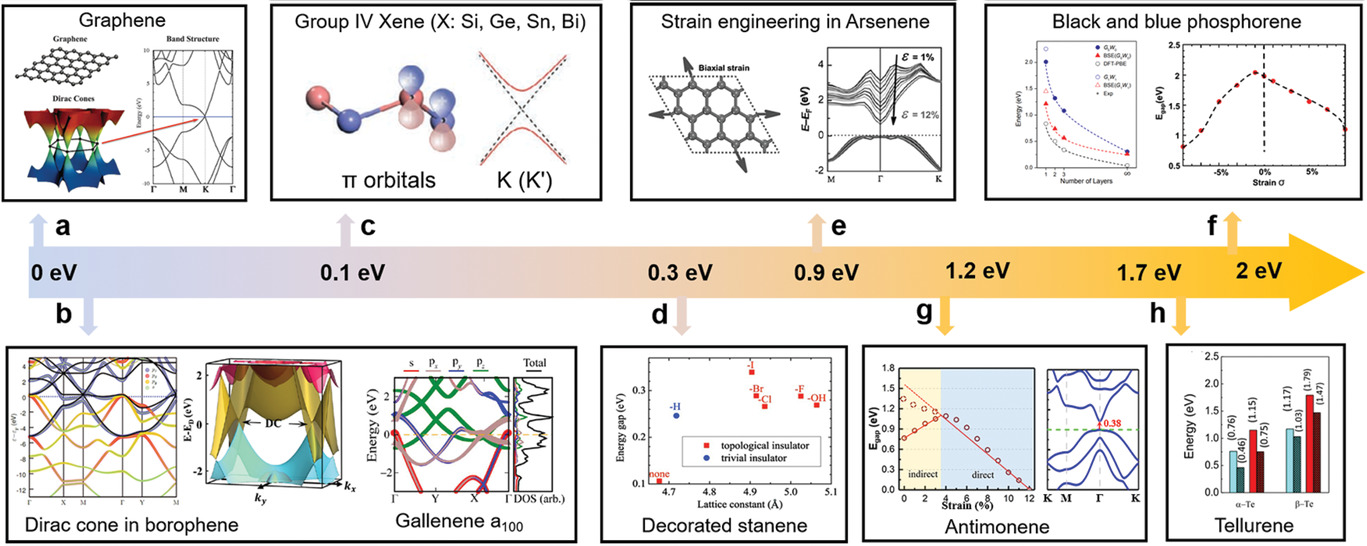
\includegraphics[width=0.8\textwidth]{pic/INTRO_electronProperties_All2DM.jpg}
        \caption{不同元素形成的多种二维材料以及二维材料体系多样化的电子特性\citing{RN1278-2021,RN903-2011}。}
    \end{figure}

    从材料性质的广度上看,多元化的二维材料赋予了二维材料器件更多,更自由的选择空间。以电子性质为例,不论是绝缘体还是半导体亦或是导体、半金属,都可以找到相对应的二维材料。
    %//电子结构
    在二维过渡金属硫化物中,以不同元素组成的二维金属硫化物材料虽然都具有相似的晶体结构,但其各自的电子性质确有很大的差异\citing{RN956-2015}。在二维过渡金属硫化物中,以六族元素硫,硒,碲和过渡金属铬,钼,钨组成的二维材料具有直接带隙,其禁带范围囊括0.5 eV至2.5 eV。而以其他六族元素和过渡金属组成的二维金属硫化物则表现出具有间接带隙的电子结构,且禁带范围扩展为0.9 eV至7.0 eV。如此宽泛的电子结构分布使得研究者可以仅仅使用二维过渡金属硫化物材料就可以组合出具有一型、二型和三型能带匹配的的半导体异质结,可用于制造包括发光二极管(一型能带匹配),单极、双极型电子器件(二型能带匹配),隧穿场效应管(三型能带匹配)等\citing{RN957-2016, RN958-2018}。

    %//光电
    多样化的的电子结构同样赋予了二维材料极宽的光响应频谱,其可以覆盖从紫外到太赫兹甚至微波的电磁波频段。当厚度逐渐减少至单原子层变为二维材料后,材料的电子性质可能会发生奇异的变化。例如,在过渡族金属硫族化合物中,MoS$_2$, WS$_2$,WSe$_2$等材料的电子结构在经过二维化后,由块体状态下的间接带隙半导体变为二维状态下的直接带隙半导体\citing{RN984-2010,RN985-2013,RN986-2015}。电子结构的变化使得二维化的MoS$_2$的发光量子效率相比于块体状态提升了4个数量级\citing{RN984-2010}。尽管只有单层或者是几层原子的厚度,二维材料独特的电子结构使其能够与光产生不同寻常的相互作用。例如单层的二维二硫化钼材料可以通过激子共振的方式吸收大约10\%的对应共振频率的光线。此外,过渡族金属硫族化合物的二维化显著降低了库伦作用的介电屏蔽效应。二维过渡族金属硫化物中较强的库伦作用大幅提高了其中激子的结合能,进而提升了材料的光响应速率\citing{RN987-2014,RN372-2013}。以单层硫化钼(MoS$_2$)为例,通过理论计算预测的其激子结合能在\SI{0.5}{\electronvolt}到\SI{1}{\electronvolt}\citing{RN989-2012,RN990-2013},大大高于传统的准二维半导体量子阱\citing{RN991-1984,RN992-1981}。而对于石墨烯而言,其布里渊区内独特的狄拉克锥电子结构导致了石墨烯具有许多独特的光电性质。例如石墨烯具有约2.3\%的宽带吸收率,使其可以作为可饱和吸收器件、光子探测器以及调制器等光电器件的候选材料。同时,包括饱和吸收效应,高次谐波产生效应,合频产生效应,四波混频效应等非线性光学效应也在以石墨烯、过渡族金属硫族化合物等二维材料体系中被发现。尤其是对于过渡族金属硫族化合物体系,其面外方向的反演对称性可通过层状堆叠打破,产生在其他二维材料无法实现的偶数次谐波效应。%//FIXME 引用
    
    \begin{figure}
        \subfloat[]{
            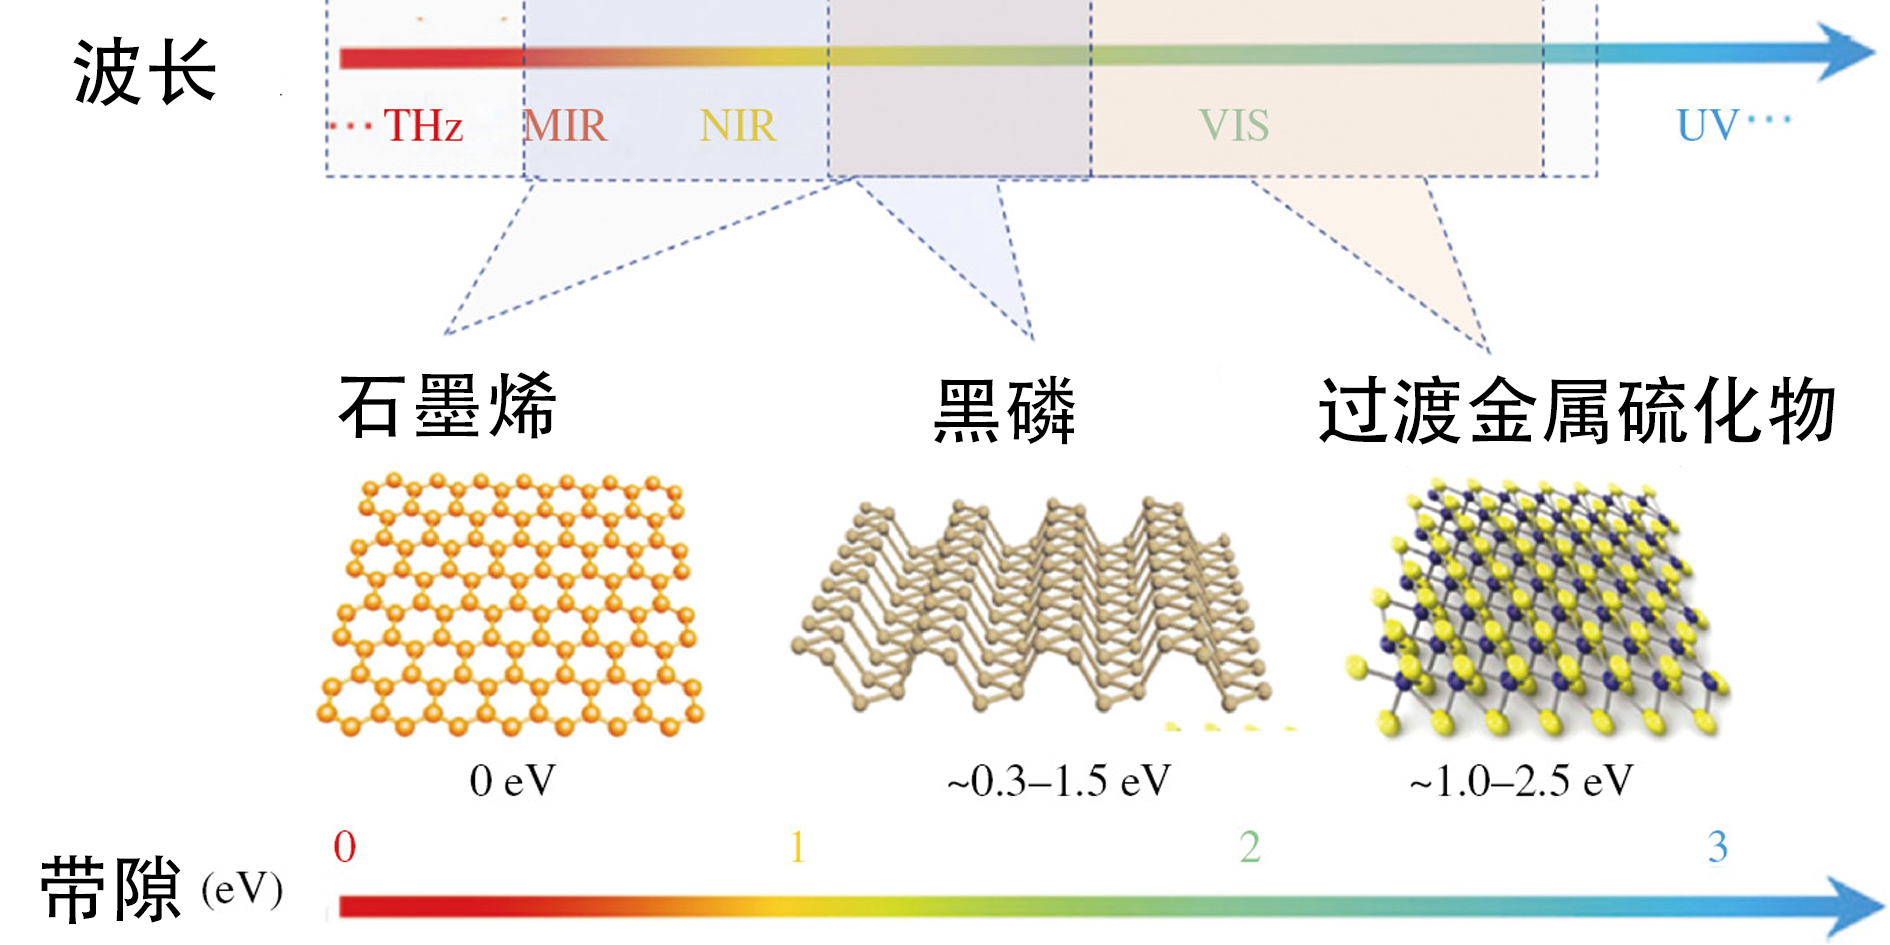
\includegraphics{pic/INTRO_optical_2D.png}
        }
        \subfloat[]{
            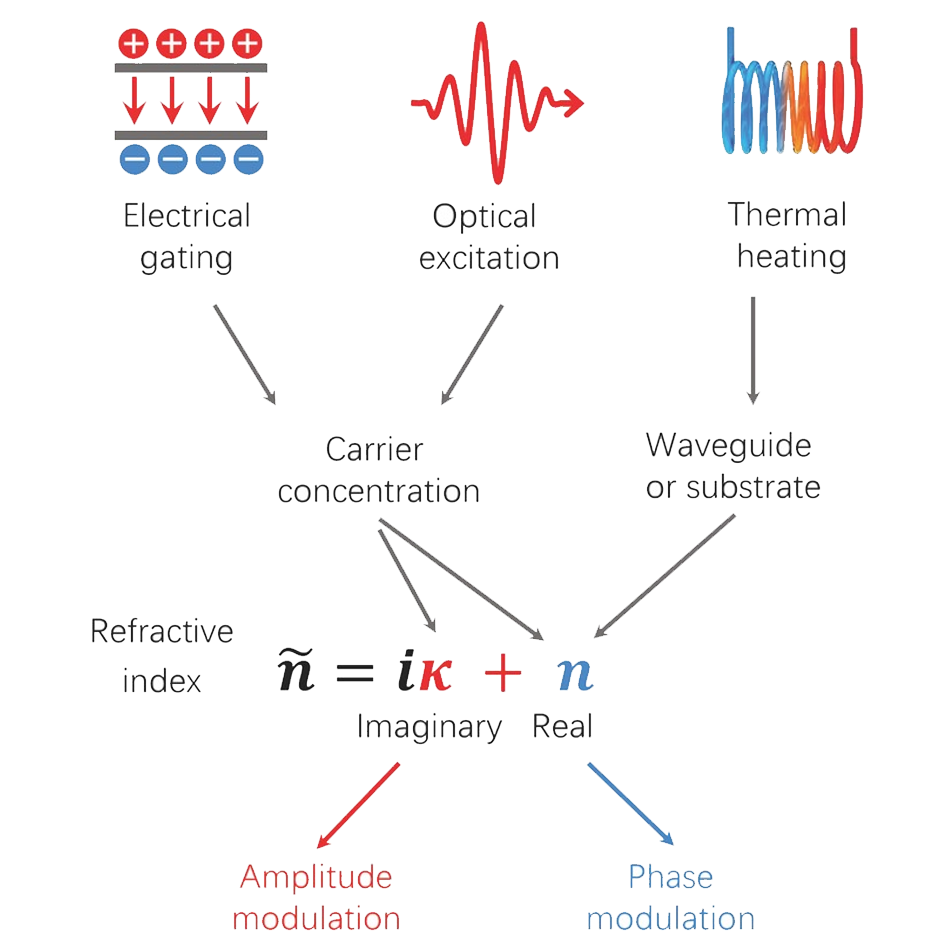
\includegraphics{pic/INTRO_optical_mechanism_2D.png}
        }
        \caption{二维材料用于光电子器件。(a)二维材料极宽的光响应频谱;(b)典型的二维材料光调制手段。}
        \label{}
    \end{figure}

    %//催化
    同样,二维材料独特的晶体结构和电子特性也引起了大量化学催化方面研究者的关注。得益于多样化并可精细调控的电子性质,利用二维材料制得的催化剂对那些对于低能级反应尤其有效,如氧气,一氧化碳,二氧化碳,甲烷,水等小分子之间的转化。这些反应对催化剂表面电子结构较为敏感,研究者可以最大可能的利用二维材料表面电子结构精细可调的优势,针对不同的催化反应对针对性的涉及二维材料催化剂。二维材料平面化的晶体结构为活性催化基团提供了精细可调的锚定位点,催化位点的电子态可以被精细调控至相应的催化底物能级,实现整体催化活性的调控。利用这样的原理,使用石墨烯,过渡金属硫化物等二维材料作为承载面,将过渡族金属原子等活性催化单元直接嵌入二维材料的平面,可以制得新能优异的单原子催化剂\citing{RN1019-2019}。在2015年,研究者通过在石墨烯表面参杂Ni制备单原子催化剂用于酸性环境下的析氢反应,其催化性能远超普通\cemb{Ni}基催化剂并且具有极高的循环稳定性\citing{RN1018-2015}。随后,通过系统的理论计算,研究者在氮参杂的石墨烯上筛选出V,Rh,Ir等金属原子作为单原子催化剂,可以显著提升析氢反应的催化性能\citing{RN1015-2020,RN1017-2019}。在2020年,有研究者报道使用ZIF8%//TODO ZIF8全称
    作为前驱体进行热熔解,可以获得具有高比表面积的Fe-N参杂石墨烯单原子催化剂,其催化性能与已经大规模商品化的Pt/C催化剂不相上下\citing{RN1016-2020}。除了石墨烯外,以过渡金属硫化物为代表的其他二维材料也作为单原子催化剂的潜在载体进入了研究者的视线。在2020年,通过使用H$_2$O$_2$对MoS$_2$进行化学腐蚀的方式,研究者在二维MoS$_2$表面获得了单S空位的催化剂,并且实现了对S空位分布的综合调控以及较强的析氢催化活性\citing{RN1020-2020}。同年,另一组研究者利用激光分子束外延的手段实现了二维CrS$_2$表面的单原子Mo参杂,CrS$_2$的表面环境极大地提升了Mo原子周围的电场水平,使得其析氢催化的性能在极大提升的同时仍然保持了较高的稳定性\citing{RN1021-2022}。
    %//FIXME 引用

    \begin{figure}
        \includegraphics{pic/INTRO_catalyst_2D.png}
        \caption{二位材料平面内单原子催化剂。}
        \label{}
    \end{figure}

    从材料性质的深度上看,二维材料同样拥有优异物理化学特性,具有非常高的应用潜力和研究潜力。在过去的十年中,二维材料所展现出的丰富的新物理激发了基础物理和技术应用方面的广泛研究。例如以石墨烯,二维过渡金属硫化物($\rm{MoS_{2}}$等) 、黑鳞(BP)等为代表的二维半导体材料具有极高的载流子迁移率和相当优异的机械性能,在下一代低功耗高速电子器件和柔性器件的制造中展现出了相当的潜力。%//TODO 引用
    同样,以六方氮化硼,金属氟化物(如$\rm{CaF_{2}}$, $\rm{TiF_{2}}$)为代表二维绝缘体材料拥有惰性的上下表面,能够很好的与其他二维材料形成范德华界面。其作为电介质层能够极大程度地减少场效应管中沟道材料的缺陷态密度,尽可能地发挥高性能沟道材料卓越的输运性能。同时,二维材料不仅能够在现有成熟器件框架下利用其优异地物理化学性质进一步提升电子器件的性能,二维材料独特的电子结构让研究者能够突破传统电子器件的限制,对电流以外的电子自由度进行操控。通过操控电子自旋进行信息处理具有速度更快、能耗更低、集成度更高以及稳定性更好的特点,研究者已经发现有许多二维材料非常适用于制造下一代高性能自旋器件。例如,石墨烯体系中超低的自旋-轨道耦合使其能够很好地保持在其上传输的自旋信息,是理想的自旋电流传输材料。而二维过渡金属硫化物体系中较强的自旋-轨道耦合性质使其能够有效地对自旋进行操控,是非常好地自旋编码材料。同时,二维材料独特的单层结构使得其电子中的能谷结构可以很容易地被附加的作用场调控,简并分裂的电子能谷作为额外的自由度可以看成赝自旋并用作信息处理的载体。自旋器件研究的兴起和器件化的推进使得这些具有自旋输运特性的二维材料体系在未来的数据存储,数据传输以及数据处理方面都有着极大的发展潜力[42]。%//FIXME 引用,语言
    %这种利用电子的自旋特性,通过对电子的自旋自由度进行操作编码来进行信息处理的自旋电子器件,由于其可编程逻辑元件和非易失性信息存储器件等不同领域的应用而备受研究者的关注。随着微加工技术和大规模集成电路的发展,电子器件尺寸进一步缩小的需求与日俱增。

    %//超导
    同时,二维材料提供了绝佳的电子结构调控平台,使得研究者能够更好地设计实验、发现新的物理现象、制造新的电子器件。而二维材料奇异的电子结构同样为新物理理论的产生提供了土壤。在二维材料中,因为具有开放的双面表面,原则上所有原子都受到表面反应的影响。同时,电荷和声子输运被严格限制在每一层中,因此其具有不同于三维体材料的特殊物理性质。以石墨烯为例,电子与蜂窝状碳晶格的相互作用使电子表现为无质量费米子,从而产生了反常的室温量子霍尔效应和极高的载流子迁移率等新的物理现象。%//TODO 引用
    在2008年,研究者测量到了石墨烯中电子的局域态分布,证实在石墨烯量子点中电子和空穴的实质上处于类似于积水潭(puddle)的存在形式。这种由于无序效应导致的新型电子-空穴分布,解释了石墨烯中零载流子密度和非零电导同时存在的现象\citing{RN998-2008}。%//TODO。
    在2012年,研究者在单层$\rm{FeSe/SrTiO_{3}}$中发现了非经典的高温超导态,揭示了在二维材料中存在传统超导理论(BCS理论)难以解释的反常超导现象\citing{RN953-2012}。而且在$\rm{FeSe/SrTiO_{3}}$系统中,超导态仅在单层$\rm{FeSe}$的情况下被发现,并且随着$\rm{FeSe}$厚度的增长消失。更加印证了在二维材料中具有有别于块体材料的超导现象。相比于$\rm{FeSe/SrTiO_{3}}$这样较为复杂的材料体系,另一个非经典超导现象在简单的石墨烯体系中被研究者所熟知\citing{RN420-2018, RN421-2018}。在扭转双层石墨烯(Twisted bilayer graphene, TBG)中,载流子的填充水平可以简单地被双层石墨烯之间的扭转角度所调控,使其能够从莫特绝缘体转变为超导体\citing{RN1068-2020,RN1071-2021,RN1065-2013,RN1067-2020,RN854-2020,RN1066-2015}。
    %//TODO 多一些转角

    %//量子计算
    同时,以石墨烯为代表的多种二维材料是天然的二维电子气载体,因此在量子计算和量子晶体管方面的应用具有独特的优势。自2007年提出可以利用二维材料石墨烯实现自旋量子比特的理论方案\citing{RN997-2007}以来,二维材料用于量子晶体管方面的研究已有较多进展。在2008年,研究者首次在二维材料石墨烯上采用刻蚀方法实现了栅极调制的单量子点结构,成功地实现了量子晶体管\citing{RN996-2008}。2009年,研究者测量了磁场调控下石墨烯量子点的电子附加能谱(Addition Spectrum)。通过对附加能谱中电子-空穴交叉的研究,研究者得到了石墨烯量子点的线性色散和边缘限制的光谱随磁场的变化情况,为石墨烯量子点电子输运行为的磁场调控提供了理论基础\citing{RN999-2009}。在2010年,自旋态以及自旋过滤现象在石墨烯量子点中测得,研究者可以通过操控外加磁场的方式调控石墨烯量子点中的自选过滤行为\citing{RN1000-2010}。在2013年,研究者成功的在石墨烯量子点中测量了激发态能级弛豫时间,证明石墨烯量子点中能级弛豫时间和GaAs等材料基本一致,都在100纳秒量级\citing{RN1001-2013}。这些一系列的研究,使我们对石墨烯以及石墨烯量子点中的电子性质的理解更加深入,更多调控手段的引入使得以石墨烯、石墨烯量子点为基础的量子晶体管的研究得到进一步发展。在2010年,研究者在石墨烯上实现了栅极可控双量子点量子器件,研究者可以通过栅极调控量子点中的电荷数量,进而调控量子点间的电子耦合特性和激子输运特性\citing{RN1002-2010}。同年,研究者通过在石墨烯大小双量子点的方式,将大石墨烯量子点作为单电荷晶体管集成在小石墨烯量子点上,并成功测量了栅极可控的小石墨烯量子点上的电荷态\citing{RN1004-2010}。在2011年,研究者成果测量了利用单、双层石墨烯制备的平行耦合双量子点的输运性质\citing{RN1005-2011},并在2012年实现了多栅极可控的石墨烯双量子点中激发态能级的测量\citing{RN1006-2012}。同年,研究者通过在空气中使用电流烧蚀的方式制得石墨烯量子点,进一步拓宽了石墨烯量子点的大规模制备手段\citing{RN1003-2012}。其高达\SI{1.6}{\electronvolt}的载流子附加能(addition energy)为同时期的最高水平,可用于制备单量子晶体管。2015年,研究者探究出了石墨烯量子晶体管和超导微波腔的色散耦合方式,并实现了量子晶体管的微波场调控\citing{RN1007-2015},以及通过维波谐振器实现的两个石墨烯量子点的长程耦合\citing{RN1008-2015}。

    这些尝试证明了在石墨烯上可以实现量子结构并进一步制成量子晶体管,但是由于石墨烯不是真正意义上的半导体,不具有直接带隙,因此在多场可调性和量子操作性上仍有一定局限。因此,近年来许多研究者开始探索以MoS$_2$为代表的二维过渡族金属硫族化物用于实现量子晶体管的可能性。
    2015年,研究者利用纵向二维异质结作为测量平台,对MoS$_2$的输运性质进行了精确测量,获得了高达34000 cm$^2$V$^-2$s$^-1$的霍尔迁移率\citing{RN993-2015}。同年,研究者在二维WSe$_2$上的实现了门定义的单量子点结构,这个单量子点的尺寸可以由相应门电极上的电压控制,隧穿势垒可由外加地电场进行控制\citing{RN1011-2015}。相比于传统的GaAs/AlGaAs异质结,该工作进一步减小了二维过渡族金属硫化物上量子点结构的尺寸,为实现更小的高性能二维量子晶体管提供了结构基础。在2016年,研究者在单层MoS$_2$上实现了单电子晶体管,并且用输运方法测量到了库伦阻塞效应\citing{RN994-2016}。2017年,研究者利用MoS$_2$和石墨烯组成的异质结实现了栅极可控的一维量子通道\citing{RN995-2017}。2017年,研究者成功测量了单层MoS$_2$在磁场中的量子输运现象及演化规律,观察到了单层MoS$_2$中量子化的电导并深入探究了MoS$_2$导带中的自选劈裂现象,并认为其可以用于制备新型二维量子自旋器件\citing{RN1009-2017}。同年,研究者在二维材料MoS2中制备了电学可调的门控双量子点结构,首次在二维材料中实现了从双量子点到单量子点的可控调节\citing{RN1014-2017}。在2018年,研究者在二维MoS$_2$中实现了门控的单量子点结构,并利用量子输运方法测量到了单电子的电荷态和激子态\citing{RN1010-2018}。同时,由于二维拓朴层状材料的发现,研究者成功的在实验中观测到了二维WTe$_2$体系中由边界态传输的量子化电导,在100K地温度下,二维WTe$_2$表现出了内部绝缘,边缘导电的奇异量子态,为量子晶体管中量子态的调控提供了新的手段\citing{RN1022-2017}。
    %利用二维拓扑体系中可用gate调控拓朴性的特点,在2D拓朴材料上实现Majorana费米子,在接下来设计复杂交换结构时仅仅需要利用半导体加工技术在材料上设计gate结构即可。

    除了优异的材料性质之外,二维材料由于其平面化的结构特点,能够较好地与与现行集成电路使用的平面硅工艺兼容。以二维材料制成的二维纳米器件能够较为容易的在现有的芯片集成,可作为新一代纳米电子器件的候选材料。

\subsection{二维材料异质结概述}
    通过将不同材料进行接触形成的异质结是许多电子器件的基本组成单原,而通过对二维材料进行纵向堆叠或者平面组装而形成的二维材料异质结能够结合不同二维材料优异的物理特性,最大化的利用其性质多样化的特点\citing{RN370-2017, RN380-2012, RN369-2014, RN371-2014, RN957-2016, RN353-2017, RN385-2014, RN351-2014, RN316-2018, RN387-2012, RN368-2017}。研究者将不同的二维材料一层层堆叠起来可以制成纵向异质结,层与层之间由较弱的范德华力或准范德华力连接。而将不同二维材料在同一层内拼接而成,不同二维材料之间通过化学键连接的异质结称为横向异质结。二维材料较弱的层间作用和相似的平面结构为二维材料异质结中稳定的界面、界线的形成提供了较好的结构基础。得益于其优秀的性质,二维材料异质结近年来发展迅速。在2010年,研究者通过将机械剥离的单层石墨烯转移到单层六方氮化硼上,首先制成了由两个单原子层的二维材料组成的异质结。在那之后,由于其独特的界面激子效应和优异的光伏相应特性,包括石墨烯/六方氮化硼,石墨烯/过渡金属硫化物,过渡金属硫化物/过渡金属硫化物在内的多种二维材料异质结引起了大量研究者的关注。迄今为止,已经有多种二维异质结通过实验合成\citing{RN961-2018, RN960-2018, RN351-2014}并用于制造场效应管\citing{RN386-2012, RN387-2012}、存储器件\citing{RN389-2013, RN388-2011}、光电器件\citing{RN390-2013}等。二维异质结使得功能更强大、特性更新颖的电子器件的出现成为了可能。

    %//二维材料异质结
    %//FIXME 修改,减少重复率
    由于机械剥离和转移技术的成熟,将二维材料进行纵向堆叠而成的纵向异质结首先进入研究者的视线。2010年,研究者通过机械剥离的方式的将单层石墨烯转移到二维六方氮化硼上,形成了具有原子层级厚度的异质结\citing{RN959-2010}。从那时起,包括石墨烯/六方氮化硼,石墨烯/过渡金属硫化物,过渡金属硫化物/过渡金属硫化物在内的大量纵向二维异质结引起了研究者的广泛关注\citing{RN309-2015, RN384-2015, RN319-2017, RN383-2012, RN368-2017},包括界面激子效应,界面磁近邻效应,谷电子效应等优异的物理性质也被逐一从二维材料异质结之中发掘出来。例如,自2015年起,已有研究者通过理论计算发现,可以将单层SnSe$_2$与单层MoS$_2$进行堆叠形成一型能带匹配的半导体异质结。其具有的超快电子-空穴复合效应使其非常适合用于制造发光二极管等光电器件\citing{RN966-2019,RN978-2017,RN979-2015}。对于二型能带匹配,由于导带底和价带顶分属于不同材料中,因此二型能带匹配可以用于电子和空穴的高效分离。若是将二维材料进行堆叠形成具有二型能带匹配的异质结,那么二维材料之间的范德华区域将对电子和空穴的相互作用产生屏蔽效应,可以对电子和空穴进行有效分离,导致其激子寿命长于普通材料\citing{RN969-2015,RN602-2015}。自2018年起,已有研究者分别从实验和理论计算的角度证实,在二维过渡族金属硫族化合物异质结,二维III-VI族化合物异质结等二维异质结体系中均可观测到持续时间非常长的电子-空穴分离态\citing{RN976-2020,RN975-2019,RN972-2017,RN977-2018}。而在二维Janus材料和二维钼硫硒化合物(MoSSe)组成的具有二型能带匹配的双原子层异质结中,在2019年,已有理论计算预测其具有长达16.5 ns的激子寿命\citing{RN971-2019}。对于具有三型能带匹配的异质结,其破缺的能带结构允许载流子在不同材料的能带之间隧穿,使其能够作为隧道场效应管的基础结构。例如,黑磷/硫化锌(Phosphorene/SnS$_2$),黑磷/硒化锌(Phosphorene/SnSe$_2$),硒化钨/硒化锌(WSe$_2$/SnSe$_2$)等材料可以组成具有三型能带匹配的异质结,已经有工作通过理论计算预测可以在这类二维异质结中观察到载流子的带间输运现象,是实现二维隧道场效应管的候选材料\citing{RN981-2018,RN982-2016,RN983-2017}。同时,由于三型能带匹配中电子和空穴的传输速度远高于二型能带匹配,大量的电子和空穴可以被迅速得分离到一直接种不同的材料上,使异质结内部产生一个较强的内建电场,并且显示出类似于半金属的特性。这样的特点使得具有三型能带匹配的异质结非常适合用于制造下一代新型热光伏太阳能电池\citing{RN980-2019}。

    不仅如此,二维材料之间的能带匹配还能够通过外加电场等方式进行改变。例如,可以在单层硒化锌(SnSe$_2$)与单层硫化钼(MoS$_2$)形成的异质结中附加外加电场,使其从原来的一型能带匹配变为二型能带匹配\citing{RN966-2019}。在单层硫化锗(GeS)和砷烯(Arsenene)形成的异质结体系中,外加正电场可以其保持原有的二型能带匹配,而外加负电场可以使其转变为一型能带匹配\citing{RN967-2019}。而在磷/硫化锌(Phosphorene/SnS$_2$)形成的具有三型能带匹配的异质结中,外加负电场可以实现一型,二型,三型的能带匹配转变\citing{RN981-2018}。除了外加电场外,最新的研究发现可以通过施加应变应力的方式,将单层硼磷化合物(Boron phosphide)和单层MoSSe形成的的一型能带匹配转变为二型能带匹配\citing{RN968-2021}。

    作为二维异质结的组成材料,引起研究者关注的不仅仅是那些具有半导体特性的二维材料。作为二维材料中的绝缘体,六方氮化硼在具有较大的带隙的同时也保有二维材料高质量面内结构的特点。趋近完美的二维晶体结构使得六方氮化硼在禁带内具有极低的缺陷态密度以及较高的击穿电压,使其能够在隧穿器件中作为非常好的势垒材料\citing{RN959-2010}。同时,利用六方氮化硼高耐压的特性,将石墨烯和六方氮化硼进行堆叠,制成的纵向二维异质结可以作为具有超薄介电层的电容器。超薄的介电层能够将小至单位电荷的变化情况传导到电极之中,使之成为量子电容器。量子电容器可用于测量量子输运体系中极其微小的电荷转移情况。运用类似的思路,将石墨烯、过渡金属硫化物以及黑磷等材料纵向堆叠成类三明治结构所制得的量子电容器也被大量研究者所关注。而最早发现的二维材料,石墨烯,其独特的电子结构使得可以通过引入外置栅极的方式对费米能级和态密度的位置进行调控,以此来操纵穿过势垒的隧穿电流的大小,适合用作隧穿器件中的源极和漏极材料。
    %\\FIXME 引用

    与传统材料界面处的共价键有所不同,纵向二维材料异质结构中各层之间相对较弱的范德华力极大地放宽了晶格匹配和化合价匹配的要求,最终实现了相比于传统材料之间更宽的异质结构匹配空间。尽管作用的强度较弱,但范德华的相互作用仍然主导了跨界面的各种类型的耦合。例如,纵向二维材料不同材料之间的电荷会在在界面处重新分布以平衡化学势,这会导致诸如电荷屏蔽、能带弯曲和载流子耗尽等现象。尽管传统的三维异质结构和二维范德华结构均发生界面电荷转移,但二者之间的电荷转移机理存在显著差异。首先,纵向二维材料异质结中范德华界面处较小的电子态交叠态,因此可以将电荷层间转移的过程限制为相对低效的隧穿和跳跃。其次,由于范德华界面处介电屏蔽的减少,导致激子结合能的增加。介电屏蔽现象消除了传统异质结中对电荷转移过程具有重大影响的能带偏移。这些因素都导致在传统异质结的理论框架下,二维材料范德华异质结中不同材料直接的电荷转移是缓慢的。但是,最近的研究发现了在部分二维材料组成的范德华异质结构中,存在超快的电荷转移过程\citing{RN595-2017, RN308-2014, RN520-2016}。研究者认为导致在范德华界面中出现超快的电荷转移过程的关键是范德华界面中激子的集体运动导致的等离子体震动\citing{RN1282-2016}。

    同时,界面耦合也会强烈地影响二维超导体的临界温度。例如,硒化铁(\cemb{FeSe})是研究最多的二维超导体之一,其体超导临界温度(Tc)约为≈8K。然而,通过在钛酸锶(\cemb{SrTiO3})上生长单层\cemb{FeSe},由于界面增强的电子-声子耦合,Tc显着提高到≈100K\citing{RN747-2014, RN746-2013, RN748-2018}。%//TODO 加一个纵向二维超导的例子
    除电子耦合外,自旋自由度的引入还导致了横向二维异质结中范德华界面的磁耦合\citing{RN1280-2019,RN1281-2020}。通常来说,相邻电子之间的自旋排列方式由自旋之间的交换作用决定。自选排序为平行或反平行对应于铁磁和反铁磁排序。通过交换相互作用和超快速电荷转移,当单层\cemb{CrI3}与\cemb{CrGeTe3}集成在二维纵向异质结中时,其中的磁有序状态会受到堆叠顺序的影响,当以AB堆叠的\cemb{CrI3}与\cemb{CrGeTe3}之间的夹角为\SI{0}{\degree}或者\SI{0}{\degree}时,\cemb{CrI3}/\cemb{CrGeTe3}异质结呈现出铁磁性,而当夹角增加到\SI{120}{\degree}或者\SI{300}{\degree}时,由于界面的磁耦合作用,\cemb{CrI3}/\cemb{CrGeTe3}异质结呈现出亚铁磁性\citing{RN1279-2020}。%//FIXME 修改 ?什么意思?

    %https://sci-hub.se/https://wires.onlinelibrary.wiley.com/doi/abs/10.1002/wcms.1353
    而对于横向二维异质结,其独特的一维界面结构使其相比于纵向异质结具有许多不同之处。相比于纵向二维异质结,横向二维异质结的边沿接触使得异质材料界限分明,有利于异质结能带匹配的调控\citing{RN568-2015}。同时,横向二维异质结中的一维边沿接触能够在原子层面提供非常小的接触面积和较低的接触阻抗\citing{RN1284-2014}。在横向二维异质结中,一维界面两边的二维材料通常以共价键相连接。共价键较强的作用力保证了横向二维异质结中界面的稳定性,同时也提升了横向异质结的光子和电子方面的器件性能。迄今为止,研究者已经成功在实验上合成了由石墨烯、六方氮化硼、过度族金属硫化物等多种二维材料组成的横向异质结,并已经用于场效应晶体管、p-n结、光电二极管、谐振器等多种电子,光电子器件的制造。

    在应用方面同样也具有广阔的前景,它们的电子特性也得到了广泛研究[29,38]。利用 MoS$_2$-NbS$_2$ 横向异质结中的交错禁带和弱耦合状态产生的传输间隙,可以制造出开关电流比为 $10^6 \sim 10^7$,漏电流约为 108 \si{\micro\ampere} 的场效应晶体管[25];利用其纳米尺寸和多组分光学性质,横向 TMD 异质结可以用作单分子探测以及制造具有可调光响应的纳米器件[39];基于 WSe2-WS2 横向异质结的 p-n 结二极管和光电二极管,表现出了良好的整流特性并能产生较大的光电流[40];这些独特的优异性能使得横向二维异质结为制造更高性能互补逻辑电路、高频器件、及光电探测器等电子、光电子器件带来了新的可能性。同时,由于横向二维异质结中普遍存在的自旋作用,进一步推动了自旋电子学和自旋器件的发展。例如 ZGNR/g-C$_3$N$_4$ 和 h-BN/graphene 构建的异质结,都有着极高的自旋过滤效率[41]。组成横向异质结的两种材料之间的界线,其进一步降低的维数还可以带来更多的激发态物理性质 [29] 。
    %//FIXME 引用,修改语言避免查重
    %//TODO 多一些横向异质结

\section{二维材料及其异质结的生长方法及生长机理}
\subsection{二维材料的生长方法及生长机理}
    二维材料以其优异的电学、光学、化学、机械特性获得了大量研究者的关注。这些新颖的特性同时也为二维材料及二维异质结带来了巨大的应用潜力和极高的理论研究价值。为了最大程度的研究了利用二维材料的诸多优异特性,研究者们一直在致力于研究二维材料及二维异质结的高质量,高可控,大规模,低成本的合成方法。一般认为,二维材料及二维异质结的合成方法可以分为两类,分别是自顶向下(top-down)合成方法和自底向上(bottom-up)合成方法。%//TODO 引用

    自顶向下合成方法是最先运用于制备二维材料的方式。在2004年,世界上第一种二维材料,石墨烯就是通过用胶带进行机械剥离的方式,从高定向裂解石墨块体中剥离而成\citing{RN1023-2004}。机械剥离可以在保留层内的共价键的同时,一步步地减弱块体材料中层间的范德瓦尔斯作用,使得单层状态的二维材料可以从相应的块体材料中分离。自2004年第一篇石墨烯被通过机械剥离的方法制备以来,机械剥离的方式在制备二维材料方面已经获得了广泛的应用\citing{RN1025-2021,RN1024-2016}。通常来说,机械剥离的方式能够制备具有极高质量的二维材料,并且可以精确地控制二维材料的层数,堆叠方式、晶向方向,旋转角度等参数,非常适合用作小规模的基础研究。虽然机械剥离是最早应用于制备二维材料的方法,但受限于较低生产效率和高昂的合成成本,剥离的方式很难应用于大规模的二维材料的生产制备。同时,机械剥离法在二维材料的制备范围上也有限制,只能制备那些具有块体异构体和层与层之间作用力较小的二维材料。为此,研究者尝试了更多成本更低,制备效率更高的剥离方式代替原本手工剥离的方法,例如化学氧化-还原法、电化学剥离法以及液相剥离法等。这些方法使用化学插层或者液相超声的方式在溶液中产生大量悬浮的单层或者少层二维材料薄片,以此来大批量地制备所需的二维材料。但通常使用化学或者超声处理对块体材料进行分层剥离的方式很难精确地控制二维材料的层数分布,同时制备的二维材料往往会因为强烈的化学作用和超声震荡引入大量的杂质和缺陷,大幅度降低制备质量。虽然这些能够进行二维材料大规模制备的剥离方式很难在那些需要精确观测电子、声子、光子作用的基础研究中施展拳脚,但已有许多研究者将其应用到了催化领域的二维材料制备之中,并取得了较好的进展\citing{RN508-2016}。

    为了克服自顶向下合成方法的缺陷,研究者探索了通过自底向上的方式合成二维材料。不同于需要相应块体材料的自顶向下的制备方式,二维材料自底向上的合成方法使用含有相应原子的前驱体,在衬底或者溶液中直接生长二维材料。使用自底向上合成的思路,已有包括物理气相沉积法(PVD)、化学气相沉积法(CVD)、原子层外延法(ALE)等方法被用于合成二维材料\citing{RN1029-2021}。虽然以物理气相沉积法、化学气相沉积法为代表的自底向上的方式合成的二维材料兼具高质量和可大规模生产的特点,但相对于机械剥离和化学剥离等自顶向下的合成方法,自底向上的合成方法通常需要如高真空、高温等更为严苛的合成环境,更加复杂的处理步骤。也因如此,二维材料的质量对自底向上合成方法的生长参数非常敏感,实验人员需要通过精确的参数调控,设计复杂的反应过程才能生长出理想的高质量大规模的二维材料\citing{RN1028-2019,RN1027-2018}。

    物理气相沉积法使用加热、离子撞击等方式使目标原子从靶材中脱离。脱离的气态原子在高真空的条件下附着在衬底上生在二维材料。针对二维材料的合成,常用的物理气相沉积法包括溅射法,分子束外延法(MBE),激光脉冲沉积法(PLD)等。其中,分子束外延法可以对生长的二维材料的层数、表面结构以及化学计量数等形貌参数加以最高精度的控制。也正因如此,为了得到更好的生长质量,分子束外延的生长速率通常较低。在分子束外延法中,原子在超高真空的环境下从克鲁森(Knudsen)容器或者电子束蒸发器中蒸发出来,沉积在基板上成核,生长城二维材料。由于超高真空的生长环境,在分子束外延的生长过程中,研究者可以通过反射式高能电子衍射(RHEED)等表面探测技术对生长中的二维材料进行原位观测,使研究者可以在生长过程中精细调控生长参数,进一步优化二维材料的生长质量。如今,分子束外延法已用于生长SnSe$_2$\citing{RN1031-2016},InSb\citing{RN1030-2016},NbSe$_2$\citing{RN1032-2021},Bi$_2$Se$_3$\citing{RN1033-2016},硅烯\citing{RN1034-2019},铋烯\citing{RN1035-2022}等二维材料。若进一步将分子束外延的蒸发装置替换为激光脉冲发射器(PLD),就能够将靶材表面在极短的时间内气化,使靶材表面产生高温高压的等离子体。这些高能等离子体扩散至衬底表面沉积生长二维材料及二维异质结。在激光脉冲沉积的过程中,激光与靶材相互作用产生的等离子体具有比蒸发器产生的原子蒸气更高的能量,因此也具有更大的扩散距离。等离子体较高的动能能够显著增强材料的二维生长趋势,使得激光脉冲沉积法能够在更低的衬底温度下生长二维材料及二维异质结。此外,激光脉冲极短的气化时间使得产生的高能等离子体具有和靶材相同的化学计量比,很大程度上能够杜绝成分优先蒸发效应,使得生长出的二维材料及二维异质结能够保持与靶材相同的成分。利用激光脉冲沉积法,研究者已经成功制备了包括石墨烯、六方氮化硼、铟硒在内的多种二维材料。%//TODO PLD 二维材料

    根据经典的薄膜生长理论,外延生长的薄膜通常表现出三种生长模式\chinesecolon Volmer-Weber生长模式(VW模式),Frank-van der Merwe生长模式(FM模式)以及Stranski-Krastanow生长模式(SK模式)。考虑二维材料的自由能$\gamma_{ad}$,衬底表面的自由能$\gamma_{sub}$以及二维材料及衬底之间界面的自由能$\gamma_{inter}$之间的竞争关系,二维材料在衬底上通常表现出FM的生长模式以及SK的生长模式。当沉积的二维材料与衬底之间有很强的相互作用时,有$\gamma_{ad}+\gamma_{inter}<\gamma_{sub}$。二维材料表现出层状生长的倾向,被称为FM模式。在异质外延系统中FM模式的出现通常意味着二维材料与衬底材料之间的较好的晶格匹配。在FM模式下,二维材料通过多点二维岛融合或者单原子台阶生长的方式进行平面化生长。通常,研究者会调整温度、前驱体种类、衬底适配程度等生长参数,将二维材料的生长模式转变为FM模式,以此进行大面积,高质量的二维材料生长。当材料与衬底之间的晶格差距较大、相互作用较弱,又具有非常高的表面能时,生长材料的表面能与界面能之和会高于衬底的表面能,此时就会表现出岛状的生长模式(VW模式),这种模式通常不利于二维材料的生长。而对于出于SK生长模式中的二维材料,单层的二维材料首先进行层状生长,形成浸润层。直到二维材料覆盖满衬底并超过临界层数后,外延生长的衬底转变为已生长的二维材料,此时生长过程中的表面能和界面能的竞争关系发生变化,展现出岛状生长的模式。由于浸润层和临界层数的存在,利用SK生长模式可以获得大规模且均匀性较高的的少层二维材料,同时也能够对二维材料生长的层数进行一定调控。%//TODO 引用

    化学气相沉积法现在已经成为以石墨烯为代表的二维材料的主要合成方法。通过精确的生长条件控制,化学气相沉积法能够在较低的成本下同时满足二维材料合成的高质量和大批量的要求。化学气相沉积法利用气态的前驱体在受控的气氛中分解,在衬底上反应生长相应的二维材料。相比于以分子束外延为代表的物理气相沉积法生长二维材料,化学气相沉积法可以既可以在低压下制备二维材料,也可以在常压下生长二维材料,同时也具有更快的生长速率。在化学气相沉积法中,由于前驱体在气相和衬底表面同步发生反应,所以衬底的选择,生长温度的变化,压力的大小,前驱体计量比的改变,甚至是衬底与生长源的距离都会对二维材料的生长演化过程,生长层数,晶粒尺寸,生长形貌以及参杂浓度等指标产生影响。以石墨烯为例,自2009年研究者首次在铜衬底上使用化学气相沉积法大规模生长高质量的石墨烯以来\citing{RN801-2009},已有多种金属衬底(Cu,Ni,Ru,Ir,Co等)被用于生长单层或者多层石墨烯。%//TODO 引用

    \begin{figure}
        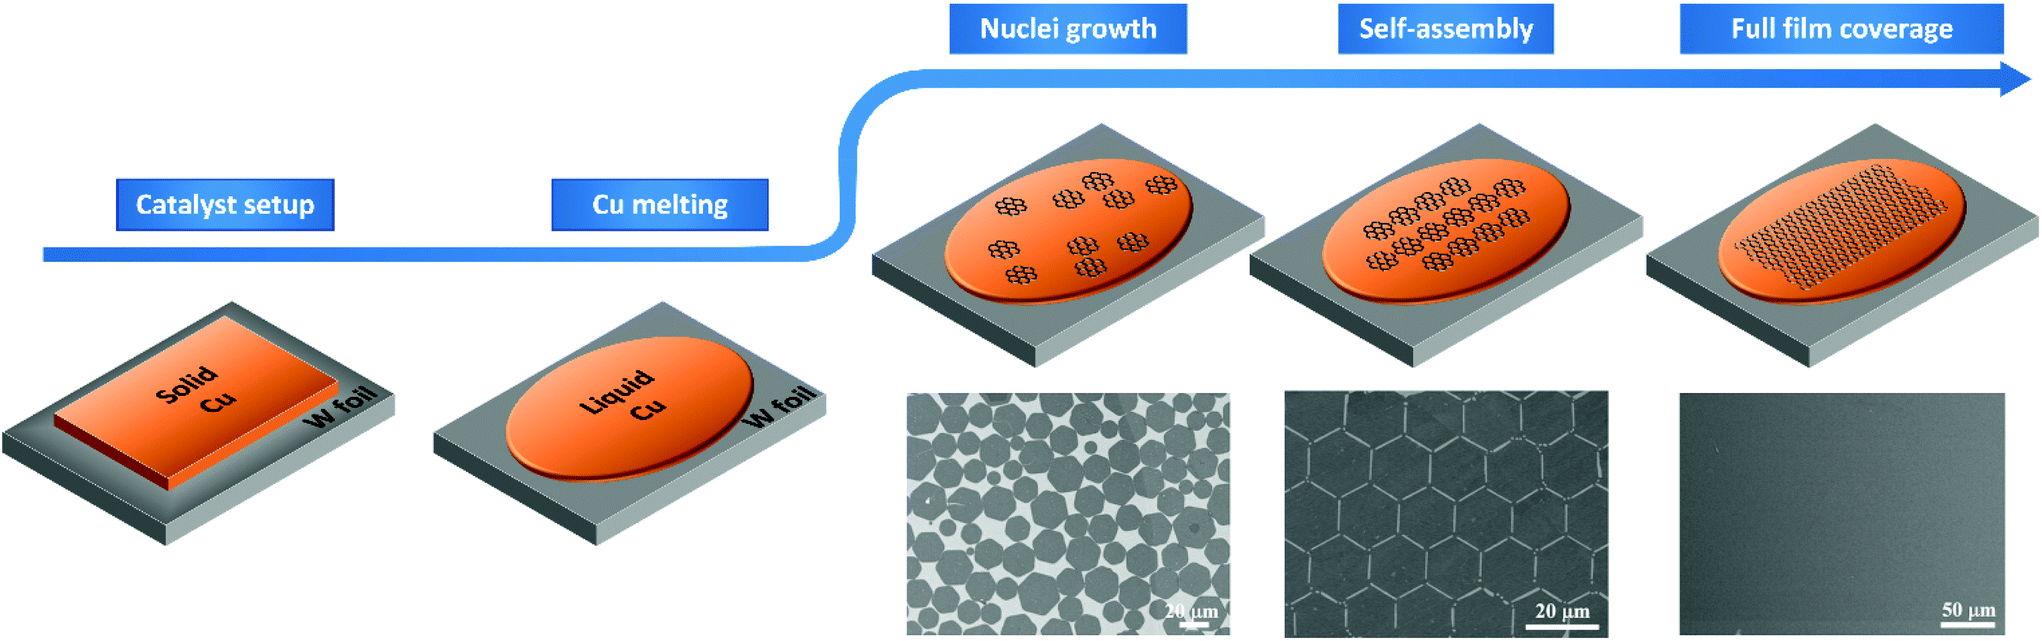
\includegraphics[width=0.8\textwidth]{pic/INTRO_CVD_graphene_growth.png}
        \caption{化学气相沉积法在金属衬底表面生长石墨烯。}
        \label{}
    \end{figure}

    衬底的选择很大程度上决定了二维材料的生长机理。通过大量的实验,研究者提出石墨烯在金属衬底上具有的两种不同的生长机制\citing{RN1041-2009}。若碳和金属之间的相互作用较弱,其在金属中就较难溶解,导致分解的碳原子只能在衬底的表面扩散生长,较容易形成单原子层的石墨烯薄膜。这种生长机制被称为扩散生长机制,通常在铜,金等衬底上体现。若碳和金属之间的相互作用较强,分解的碳原子会进一步溶解进金属衬底中,在衬底的表面上形成一层金属碳化物合金。这部分碳原子会在生长过程中向衬底表面偏析,从而形成石墨烯多原子层。这种生长机制被称为沉淀生长机制,通常在镍,钴,钌等金属衬底上有所体现。同时,用于石墨烯生长的主要直接碳源也取决于金属衬底的种类以及生长的温度\citing{RN1050-2015}。由于含碳前驱体的不完全裂解,石墨烯在衬底表面的成核密度随着温度的上升而上升,石墨烯生长的直接碳源也会随着温度的变化而变化。在\SI{800}{\kelvin}的生长温度下,研究者发现生长在铜(111)表面和镍(111)表面的石墨烯的主要碳源为次表面碳和表面\cemb{CH}自由基\citing{RN828-2012}。而当温度上升至\SI{1400}{\kelvin}时,由于含碳前驱体在金属衬底表面进一步裂解,石墨烯的生长直接碳源变为表面碳和次表面碳。
    金属衬底对前驱体的催化作用极大提升了二维材料的生长速率,并且有利于实现二维材料生长过程中的层数控制,但从金属衬底上生长的二维材料通常需要被转移到绝缘材料上才能够进一步的与现有硅基半导体工艺技术结合,制成晶体管等电子器件。这样的转移过程很可能会对二维材料的质量造成影响,使其器件能下降。因此,若绝缘衬底上直接生长二维材料,就可免去了转移的步骤,使得二维材料能够更容易的集成进现有半导体工艺步骤之中。2011年起,研究者相继实现了化学气相沉积法石墨烯在蓝宝石\citing{RN1042-2013}、二氧化硅\citing{RN1043-2011}等绝缘体表面的生长制备,进一步提升了二维材料的集成器件化水平。

    而前驱体在化学气相沉积的过程中作为反应物,经过热解反应、气相化学反应、组分输运过程,在衬底的表面转化为二维材料。由于化学组成的差异,不同的二维材料所需的前驱体相距甚远,使用不同的前驱体生长的同一种二维材料也具有不同的生长机制。例如,氢气、甲烷的组合通常用于生长高质量的石墨烯,其流速流量可精确调控的特性可以让研究者很方便的对生长中的石墨烯进行尺寸、形态和结构的控制,同时在氢气环境下甲烷裂解不会产生额外的副产物,保证了石墨烯生长碳源的纯度。事实上,各种含碳化合物都有被用来研究通过化学气相沉积法合成石墨烯,包括乙烯、乙炔等气体,也包括乙醇、苯、戊烷等液体,以及PMMA等固态前驱体。%//TODO 机理,引用
    不同的含碳化合物在化学气相沉积的过程中具有不同的解离过程,而碳前驱体的解离是化学气相沉积法制备石墨烯的关键步骤。虽然在传统的化学气相沉积生长石墨烯的机理研究中,甲烷在气相中的反应由于其非常高的脱氢势垒(大约为$4.8\si{\electronvolt}$)被大多研究者所忽略。但由于石墨烯的化学气相沉积生长通常需要极高的温度(通常在1000 K左右),甲烷在气相反应中脱氢裂解产生CH$_3$等自由基的影响变得不可忽略\citing{RN829-2012}。也正因为前驱体在化学气相沉积过程中的反应路径对石墨烯等二维材料的生长起了非常大影响,研究者引入了其他活性物质来进一步调控化学气相沉积中二维材料的生长过程,以此来控制二维材料的形貌,提升生长质量。同样以石墨烯为例,除了含碳前驱体外,研究者还通过引入如氢气,氧气等能够参与含碳前驱体解离和反应过程的物质参与到生长过程之中。通常,氢气会影响金属衬底表面活性碳分子的吸附过程,并且会在生长过程中与石墨烯的边缘结合,甚至会腐蚀石墨烯。在氢气含量较低时,石墨烯的边缘倾向于与金属衬底表面成键。在这种情况下,游离在金属衬底表面的活性炭分子可以较为容易地和石墨烯地边缘成键,进一步对石墨烯进行生长,形成单原子层的石墨烯晶畴。而当氢气的含量较高时,氢原子会与石墨烯的边缘结合,使得石墨烯边缘与金属衬底分离。在这种情况下,金属衬底表面游离的活性碳分子就会进入石墨烯与衬底的界面处,并形成新的石墨烯畴。这样的过程会导致石墨烯倾向于生长出双层、多层的形貌。由此,研究者便可以通过调控生长环境中氢的含量来实现石墨烯生长的层数控制。%//TODO 引用
    同样,氧气的引入也对石墨烯的成核及生长既有显著的影响。2011年,研究者发现铜衬底表面的吸附氧能够显著降低甲烷分子解离反应的反应势垒,而镍,铑,铱等衬底的表面氧则倾向于提高甲烷的解离难度\citing{RN1051-2011}。研究者也发现氧原子的存在同时能够促进铜衬底上双层石墨烯的生长。铜衬底表面的氧原子提升了铜的次表面对于活性炭的溶解度。理论计算显示在表面有氧原子的情况下,铜衬底次表面处碳原子的能量比石墨烯-铜衬底界面处低大约\SI{0.6}{\electronvolt}。次表面的碳原子容易再次偏析,从而为在界面处生长的第二层石墨烯提供碳源\citing{RN1052-2016}。

    而对于二维过渡族金属硫化物,通常使用硫前驱体直接对过渡金属或者其氧化物衬底表面硫化的方式,在衬底的表面形成单层或者几原子层的二维过渡族金属硫化物纳米片\citing{RN1045-2012}。也有研究者使用挥发性过渡族金属氧化物和硫前驱体共蒸发的方式,前驱体蒸气经过气相反应后,在衬底表面沉积形成二维过渡族金属硫化物纳米材料\citing{RN1046-2018}。同时,研究者也一直在改进化学气相沉积技术来进一步提升二维材料的生长质量。2014年,研究者在石墨烯的化学气相沉积生长过程中引入等离子体增强技术,提高沉积原子的动能,降低石墨烯生长过程中对衬底温度的要求,从而减少衬底的污染\citing{RN1047-2014}。2016年,研究者发现可以将气态前驱体局部地引入衬底表面,使石墨烯在衬底表面成核位置限制在一点,从而快速生长单原子层的石墨烯单晶\citing{RN1044-2016}。

%参考
%https://sci-hub.se/10.1088/1361-6633/aa9bbf
%//TODO https://sci-hub.se/10.1038/s41570-016-0014

\subsection{二维材料异质结的生长方法及生长机理}
    将具有不同电子、光电特性的二维材料进行组合,可以制成二维材料异质结。通过将二维材料进行纵向堆叠或者横向拼接,利用各种方法制备的纵向和横向二维异质结展现出了优异的器件性能以及新颖的物理特性。

    %%纵向二维异质结
    对于纵向二维异质结,与二维材料的制备方法类似,机械剥离与转移的方法首先被应用在石墨烯/六方氮化硼的纵向异质结构的制备之中\citing{RN959-2010}。在这之后,研究者进一步改良了机械剥离法对于二维纵向异质结的制备。例如在2011年,研究者通过引入光学掩膜的方式对机械剥离石墨烯的转移技术进行改进,大幅改善了转移后石墨烯的平坦度\citing{RN1053-2011}。由于操作简单,合成质量较高的优点,机械剥离法同样也被成功用于石墨烯/过渡金属硫化物等纵向二维异质结的制备\citing{RN390-2013}。

    对于纵向异质结的合成,机械剥离的方式仍然受低合成效率的限制。为了突破机械剥离方法的局限,研究者开发了多种方法通过在二维材料上直接生长另一种二维材料来制备纵向二维异质结。例如,利用
    分子束外延法具有的连续交替生长多层材料能力,能够非常适合生长非常高质量的二维材料异质结。例如在2015年,研究者通过在分子束外延法在外延石墨烯上直接生长单层MoSe$_2$,制得MoSe$_2$/石墨烯纵向异质结\citing{RN1036-2015}。在2016年,研究者在六方氮化硼上生长出了高质量的单层MoSe$_2$,并且实现了功函数的调控\citing{RN1037-2016}。

    在二维材料生长中大显身手的化学气相沉积法也被用于直接生长纵向二维异质结。在2011年,研究者利用化学气相沉积法在六方氮化硼单晶上直接生长出了多层石墨烯\citing{RN1056-2011}。虽然六方氮化硼单晶不规则的表面对生长石墨烯的质量造成了一定的影响,但直接在六方氮化硼上生长层数可调的石墨烯将纵向二维异质结的大规模制备提升到了新的高度。随后,研究者通过小碳流的方式,将石墨烯的沉积反应控制在稳态附加,使得碳原子能够尽可能地在石墨烯畴的边缘生长,最终在氮化硼的表面实现了面积约\SI{11}{\micro\metre}的石墨烯单晶\citing{RN1058-2014}。但是,由于六方氮化硼对于甲烷等含碳前驱体裂解反应的催化活性远不及金属衬底,石墨烯在六方氮化硼上直接生长的速率同样也远低于在金属衬底上的生长速率。因此,一些研究者试图通过增加前驱体裂解速率的方式提升纵向二维异质结的合成效率。例如,研究者发现可以通过添加作为气体催化剂的硅烷等方式,可以促进甲烷的裂解,由此大大提升石墨烯在六方氮化硼上的生长速率\citing{RN1059-2015}。通常来说,对于使用两步法进行纵向二维异质结的制备时,首先需要尽可能地提高第一层二维材料的制备质量。高质量的第一层二维材料有利于降低后续材料的成核密度,提高晶畴尺寸\citing{RN1267-2020}。而在2015年,研究者发现一种通过控制原子在金属衬底中扩散行为的方式,利用夹层原子源,在金属衬底的表面产生共偏析的现象,成功在\cemb{Ni}衬底的表面生长出了大面积的石墨烯/六方氮化硼纵向异质结\citing{RN1271-2015}。
    
    化学气相沉积法同样由于生长二维过渡族金属硫化物所组成的纵向异质结。一步法化学气相沉积法是生长二维过渡族金属硫化物所组成的纵向异质结的有效方法。在2014年,研究者利用MoO$_3$和钨不同的蒸发温度,以粉末状的钨,MoO$_3$以及硫作为前驱体使制备了WS$_2$/MoS$_2$纵向异质结\citing{RN369-2014}。在2016年,研究者利用W原子和Re原子在不同表面吸附能力的差异,使用在金衬底上制备了ReS$_2$/WS$_2$纵向异质结\citing{RN1119-2016}。在2017年,研究者通过调控输入气体\cemb{CH4}流量的不同,控制\cemb{Mo}-\cemb{Cu}合金衬底上生长\cemb{MoC2}和石墨烯的速度,从而实现\cemb{MoC2}/石墨烯纵向二维异质结的生长\citing{RN1272-2017}。
    对于生长包含二维过渡族金属硫化物的纵向二维异质结的另一种有效的方法是现在已生长的二维材料上沉积前驱体,通常为对应二维过渡族金属硫化物的金属层或者金属氧化物层。接着,再在生长氛围中通入如\cemb{H2S}等硫族化合物对已沉积的前驱体层进行硫化,达到在指定二维材料上方大面积合成二维过渡族金属硫化物的目标。在2019年,研究者就通过这种先沉积,后硫化的方法制备了大面积的\cemb{MoS2}-\cemb{graphene}异质结\citing{RN1268-2019}。这种先沉积,后硫化的方法也可以在生长过程中多次使用,即可生长不同二维过渡族金属硫化物堆叠而成的纵向二维异质结。在2016年,研究者通过多次先沉积,后硫化的方法,使用过渡金属作为沉积前驱体,制备了九层堆叠的\cemb{WS2}/\cemb{MoS2}二维纵向异质结\citing{RN1269-2016,RN1270-2016}。

    而对于横向二维异质结,机械剥离法很难将不同的二维材料进行同一平面内的拼接。因此,研究者的目光集中在能直接生长二维材料的化学气相沉积法和物理气相沉积法。对于平面内接合的横向二维异质结,分子束外延法也能够进行较高水平的生长。在2020年,研究者在\cemb{Ag(111)}衬底上实现了锗烯/锡烯横向二维异质结的连续生长\citing{RN1038-2020}。同样,石墨烯/六方氮化硼横向二维异质结也被发现能够通过分子束外延的方法进行高效制备\citing{RN1039-2020,RN1040-2021}。尽管能够生长非常高质量的具有原子级清晰界面的横向二维异质结,利用分子束外延生长横向异质结的方法同样受困于较高的真空要求、较低的生长速率以及高昂的成本。因此,许多研究者致力于对化学气相沉积法生长进行改进,以期能够快速低成本的生长横向二维异质结,进一步促进横向二维异质结的器件化和产业化。
    在2010年,研究者通过一步气相沉积法合成了石墨烯/六方氮化硼横向异质结\citing{RN114-2010}。而对于以二维过渡族金属硫化物组成的横向二维异质结,还可以通过将单层二维过渡族金属硫化物中部分边缘层进行化学转化的方式,制成相应的横向异质结。例如在2018年,研究者通过对\cemb{MoS2}的边缘进行加氢脱硫以及碳化的方式,成功制成了\cemb{Mo2C}/\cemb{MoS2}二维横向异质结\citing{RN1275-2018}。

    这种通过一步化学气相沉积法合成的横向异质结质量较低,同时在空间分布上难以进行人为控制。由于一步合成的方法基于材料的自组装,研究者很难对二维横向异质结的形状和尺寸进行精确调控。同时对于过渡族金属硫化物体系,倘若异质结内不同材料中的过渡金属和硫族元素同时发生了变化,一步法很难生长如同WSe$_2$/MoS$_2$ 这样的异质结。为了克服一步法生长横向二维异质结的困难,在2012年,研究者发展出了通过两步化学气相沉积法对石墨烯/六方氮化硼横向异质结进行合成\citing{RN}。在两步法中,研究者发现六方氮化硼倾向于在已生长的石墨烯边缘优先成核,因此可以将二维横向异质结的生长范围限制在石墨烯边缘。2013年,研究者使用改进的两步化学气相沉积法合成了具有原子级清晰界面的石墨烯/六方氮化硼横向异质结\citing{RN}。2015年,有原子级的清晰界面的WSe2/MoS2异质结通过两步外延生长方法成功合成\citing{RN568-2015}。在2021年,研究者发现,可以通过调控前驱体中\cemb{Se}/\cemb{W}的比例,利用\cemb{WSe}和\cemb{WSe2},精确控制双层\cemb{WS2}/\cemb{WSe2}横向异质结中第二层\cemb{WSe2}的生长\citing{RN1274-2022}。

    在大规模的合成中,纵向异质结和横向异质结的合成方式通常具有很高的相似性。很多时候研究者需要通过利用不同的生长机制,使得二维材料在反应过程中专注于纵向生长或者横向生长。例如在2017年,研究者利用\cemb{CH4}前驱体在\cemb{MoC2}和石墨烯表面吸附能力的差异,使得\cemb{CH4}前驱体在\cemb{MoC2}的表面优先吸附,避免了碳源在石墨烯或者催化衬底表面反应,参与到\cemb{MoC2}的横向生长之中。在2019年,研究者通过设计调控前驱体中\cemb{W}元素和\cemb{Se}元素的比例,控制气相中的\cemb{W_xSe_y}分子团簇类型,利用不同\cemb{W_xSe_y}分子团簇在\cemb{MoS2}表面动力学行为的不同,控制\cemb{WSe2}的成核位点,达到控制\cemb{WSe2}在\cemb{MoS2}边缘生长和在\cemb{MoS2}上表面生长的切换的目的,实现\cemb{MoS2}/\cemb{WSe2}横向或者纵向异质结的切换生长\citing{RN1273-2019}。在2020年,研究者通过氢氧化物辅助的策略,通过控制生长温度的方式控制\cemb{WS2}的成核位点,达到\cemb{WS2}/\cemb{MoS2}的横向和纵向异质结切换生长的目的\citing{RN1276-2020}。
\section{本论文研究的主要思路及内容}
%//TODO 本文的主要研究思路